% !TEX encoding = UTF-8 Unicode

\documentclass[twocolumn,10pt,a4j]{ltjsarticle}
\usepackage{kougai}

\title{個人でのVR技術の利用状況}
\author{1932131 三原 巧巳  指導教員 須田 宇宙 准教授}
\date{}

\begin{document}

\maketitle

\section{はじめに}
近年,xR(AR,MR,VR)技術の発展やコンテンツが増えたことにより,私たちの日常生活の中でも見かける機会も増えている.
現在,AR技術とMR技術を利用するにはスマートフォンやスマートグラスなどが用いられ,技術を利用するにはスペースをあまり必要としていないことが多い.
AR技術はスマートフォンを利用したコンテンツが多く存在し,MR技術は工業や医療の場で多く利用される.

一方,VR技術を利用するには,専用のヘッドマウントディスプレイを装着した上で動き回るため,コンテンツによっては大きな機材や広い場所も必要となる.
VR技術は,ゲームやアトラクション施設の場で利用されることが多いが,数は少ないというところが問題である.
これからも普及率が低い場合VR技術が発展していかなくなってしまうおそれがある.
技術が発展していかなかった場合エンターテイメントの幅が広がらないだけではなく,現実では危険な実習や現実には起こしづらい現象の体験が困難である.

本研究では,普及しない理由はコンテンツにあると仮説を立て,それを元にVR機器の普及度と,購入されている種類・傾向,および購入していない人に対して,購入していない理由などについて調査をすることを目的としている.

\section{xRについて}
ARとは,「Augmented Reality」の略称であり「拡張現実」とも呼ばれている.
カメラで現実世界を映し,その上にCG映像や文字情報を重ねる技術である.
%ARコンテンツを利用するためには,専用の機材を必要とせず携帯端末などで利用することができる.

MRとは,「Mixed Reality」の略称であり「複合現実」とも呼ばれている.
カメラを通して現実世界を認識し,実写とCG映像や文字情報を重ねることで現実世界と仮想世界を融合させる技術である.
%MR技術を利用するには,専用のデバイスやカメラだけではなく,仮想世界で作られたものを映すためのマーカーなども必要となる.

VRとは,「Virtual Reality」の略称であり「仮想現実」とも呼ばれている.
VR専用のゴーグルを装着して,視界全体に映像を映すことで自分が映像の中に入り込んだような体験ができる技術である.
さらにVRの中で移動やものの操作などができ,現実に近い体験から非現実的な体験まで幅広くが扱うことができる.
%VRコンテンツを利用するためには,専用のゴーグルと専用のコントローラーなどが必要となる.

%図1に示すように2021年ではVRを認知している人は90%もいるが,実際に利用したことある人は全体の17%のみであり,継続して利用していたのは5%という結果からVR技術はあまり普及していない[1].

%\begin{figure}[h]
%\begin{center}
% 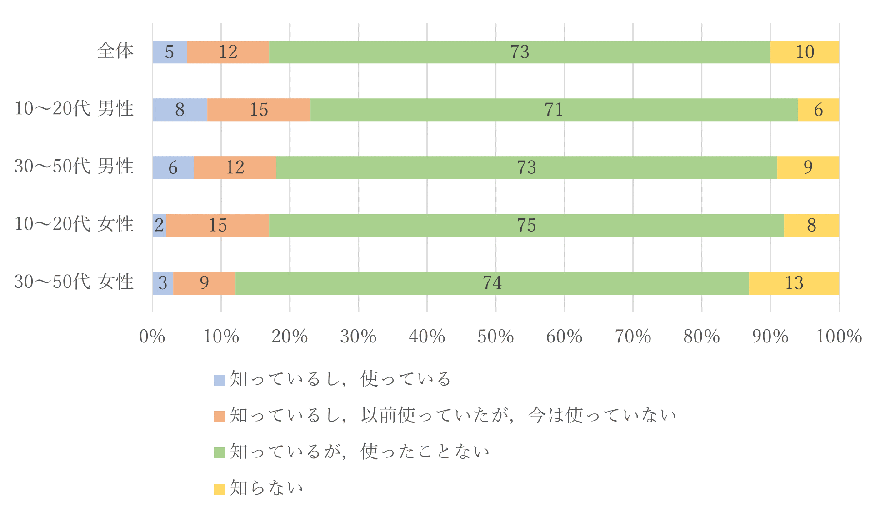
\includegraphics[clip,width=85mm,height=55mm]{グラフ_0903.pdf}
%\end{center}
% \caption{VRの現状}
% \label{fig:比較グラフ}
%\end{figure}


\section{調査について}
現在,VR機材には高い機器もありその機器を利用したコンテンツもあるが,ほかのゲーム機器やスマートフォンなどと比べると金額の差はさほどない.
VRコンテンツが普及しない理由として長期間かつ多くの人に人気になるようなコンテンツがないという仮説を立てた.

本研究では,Google Formsを利用してアンケートを2回行った.アンケートの対象として,千葉工業大学の学生を対象とする.
1回目のアンケートでは,VRを体験したことある人と体験したことがない人,VR機器を所持したことがある人と所持したことがない人で分け,VRに求め手られているコンテンツやどのような目的で購入されたかなどを調査した.
2回目のアンケートでは,主に機材についての質問とコンテンツについて質問をして,どのような機材やコンテンツがあると普及するかという調査をした.

今回の調査で分かったことは図\ref{fig:vr機器を所持するまでに至らなかった理由.pdf}から購入に至らない理由として機材の価格が高いということである.
また,コンテンツでは図\ref{fig:購入したいと考えたvrコンテンツ.pdf}から有名タイトのVR化よりVRを感じやすいコンテンツが求められていることが分かった.

\begin{figure}[h]
\begin{center}
 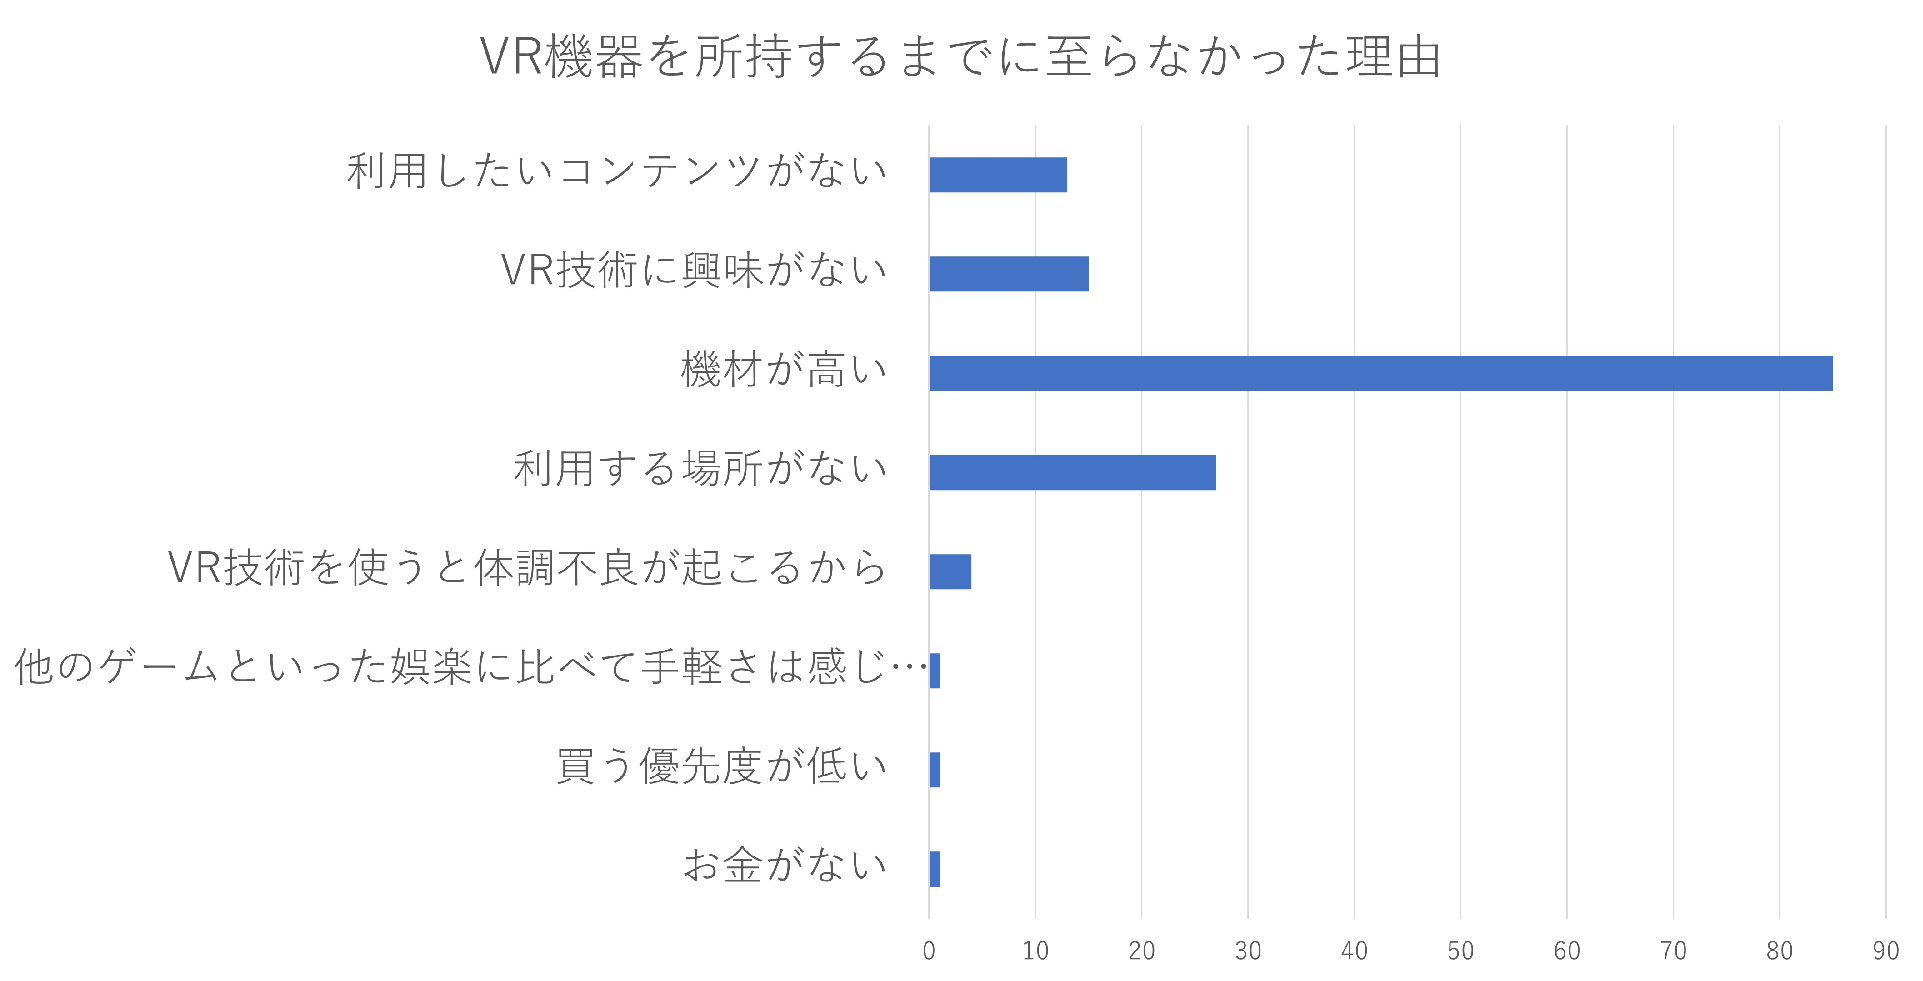
\includegraphics[clip,width=85mm,height=55mm]{vr機器を所持するまでに至らなかった理由.pdf}
\end{center}
 \caption{VRの現状}
 \label{fig:vr機器を所持するまでに至らなかった理由.pdf}
\end{figure}

\begin{figure}[h]
\begin{center}
 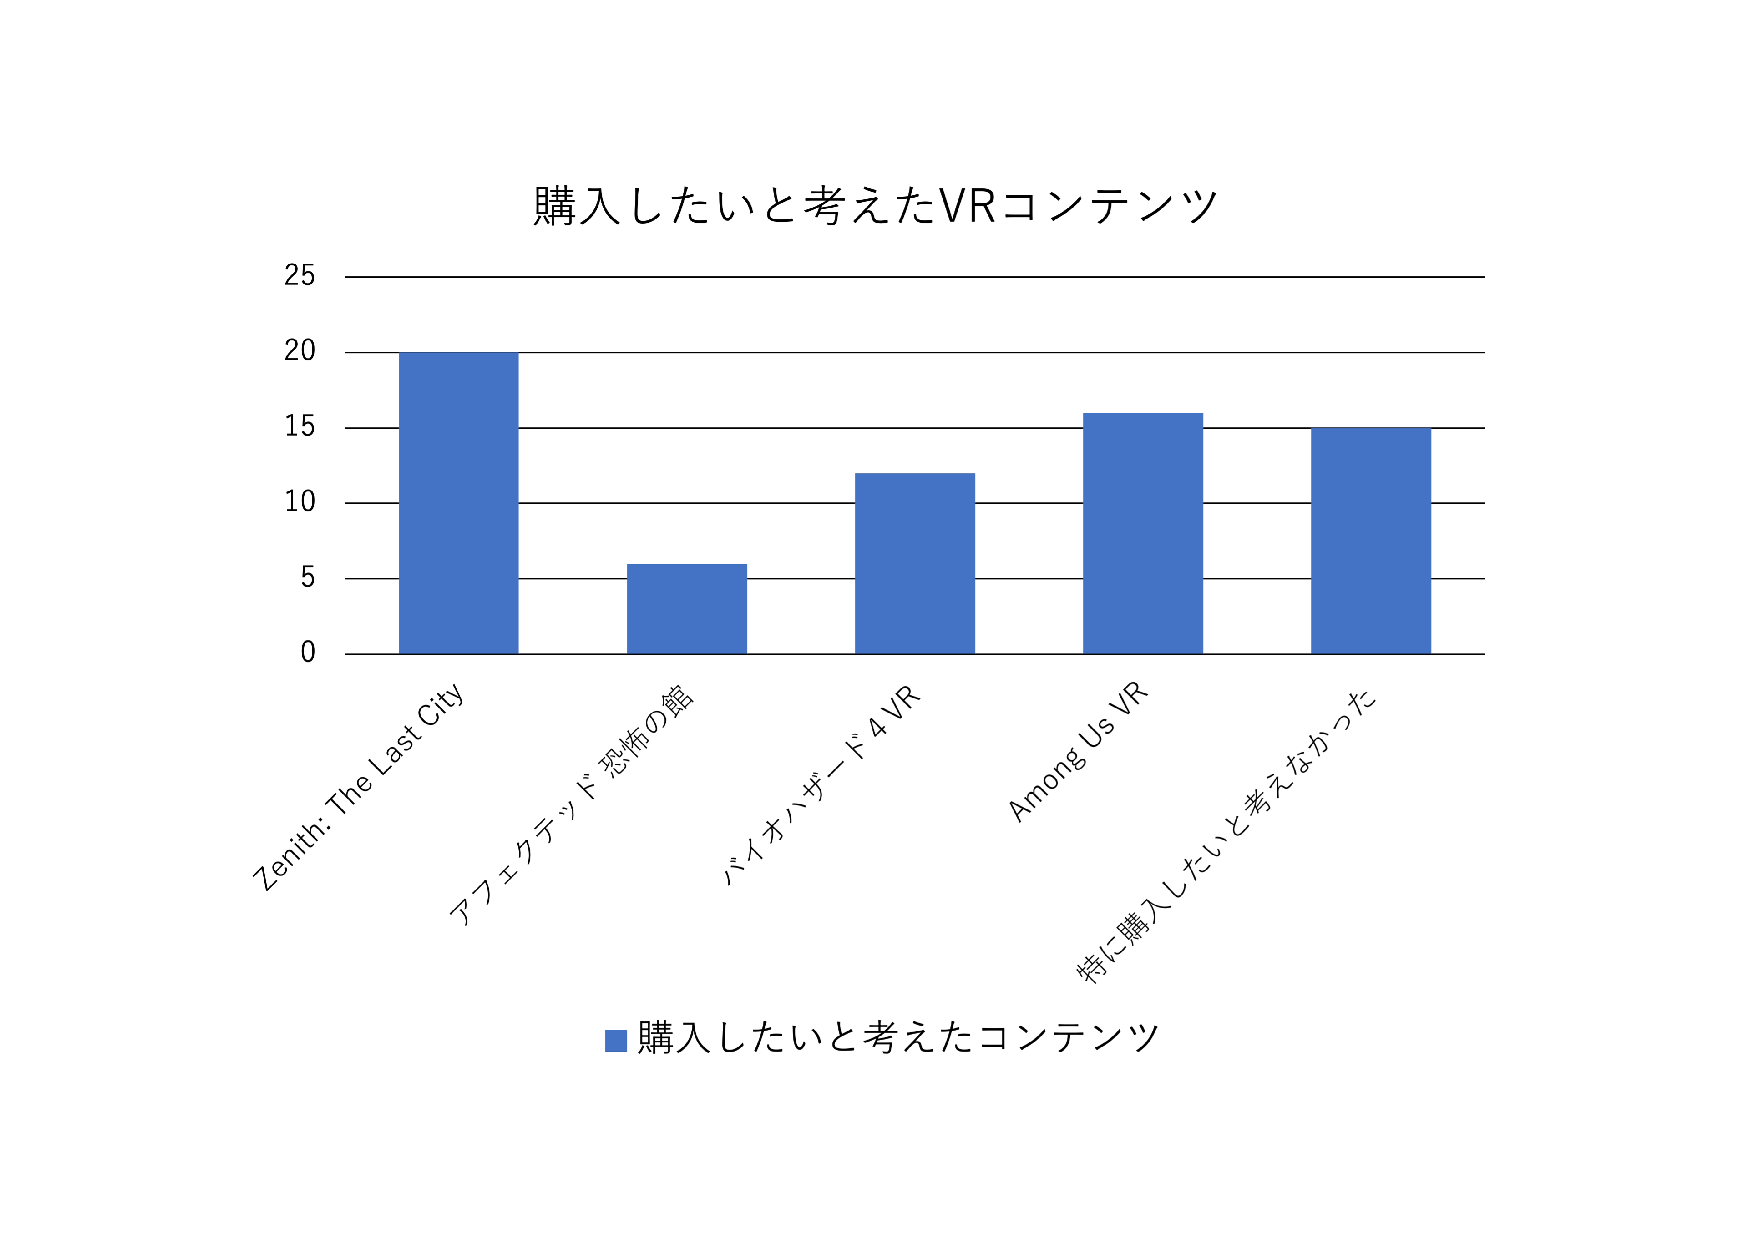
\includegraphics[clip,width=85mm,height=55mm]{購入したいと考えたvrコンテンツ.pdf}
\end{center}
 \caption{VRの現状}
 \label{fig:購入したいと考えたvrコンテンツ.pdf}
\end{figure}

\section{おわりに}
今回調べた結果VR機材のコストが低くなる普及すると考えている.
その理由として,今回のアンケートで大学生が求められているコンテンツでは既存のもので十分に行えるが機材が高価なため購入をしないと考えている人が多いことから考えられる.

%\begin{thebibliography}{99}
%\bibitem{VR}  ``流行体感から読み解くサービス未来予測 流行予想シリーズ ~VR(バーチャルリアリティ)編~'', \url{https://research-platform.line.me/archives/38203466.html}, 2022/9/2参照
%\end{thebibliography}

\end{document}
